\mode<presentation>
{
  \usetheme{CambridgeUS}
  \usecolortheme{whale}
  \usecolortheme{lily}

  \setbeamercovered{transparent}
  \usefonttheme[onlymath]{serif}
}

\title[\NyquistStabilityTheoremShortName] % (optional, use only with long paper titles)
{\course: \NyquistStabilityTheoremName\license}

\subtitle
{Lecture \NyquistStabilityTheoremNumber} % (optional)


% Delete this, if you do not want the table of contents to pop up at
% the beginning of each subsection:
%\AtBeginSection[]
%{
%  \begin{frame}<beamer>{Outline}
%    \tableofcontents[currentsection,currentsubsection]
%  \end{frame}
%}


% If you wish to uncover everything in a step-wise fashion, uncomment
% the following command:

%\beamerdefaultoverlayspecification{<+->}


\begin{document}

\begin{frame}
  \titlepage
\end{frame}

\mode<article>{
\maketitle
\tableofcontents
}

%\mode<presentation>{
%\begin{frame}{Outline}
%  \tableofcontents
%  % You might wish to add the option [pausesections]
%\end{frame}}
\section{Another Stability Test?}

One of the most important characteristics of a feedback control system is that it is {\em stable}. Thus far, we have checked stability of a feedback system by finding the closed loop transfer function and checking to see if any poles are in the right half plane. 

\begin{frame}{Checking Stability, so far...}
\begin{center}
\input{figures/feedbacksystem.tex}
\end{center}
\[
T(s) = \frac{N(s)}{D(s)} \quad \quad D(s)=0\mbox{ for } \mbox{Re}(s)>0?
\]

\end{frame}

%We developed the Routh-Hurwitz test to help us check for stability by hand. 
In this lecture, we will develop another stability test for feedback systems that utilizes the frequency response of the loop gain, $G(j\omega)$. That is, given the frequency response of the {\em open loop system} we can {\em predict} if that system would be stable with unity gain feedback applied. This test will be especially useful when there is some uncertainty to the exact value of $G(j\omega)$, making it valuable for checking the robustness of a control system to variations in the system to be controlled.

\section{The Nyquist Stability Test}

The Nyquist stability test checks for stability of a \textit{closed-loop} system 
\[
T(s) = \frac{Y(s)}{R(s)}
\]
using the loop gain $L(s)$, which is simply the product of all of the individual transfer functions around the feedback loop:
\begin{frame}{Loop Gain}
\begin{center}
\input{figures/loopgain.tex}
\end{center}
\mode<presentation>{\[
\frac{Y(s)}{R(s)} = \frac{G(s)C(s)}{1+C(s)G(s)H(s)} = \frac{G(s)C(s)}{1+L(s)}
\]
}
\end{frame}

Note that for the above feedback system the closed loop system transfer function is 
\[
\frac{Y(s)}{R(s)} = \frac{G(s)C(s)}{1+C(s)G(s)H(s)} = \frac{G(s)C(s)}{1+L(s)}
\]
The poles of the closed loop system will be the values of $s$ such that $L(s)=-1$\footnote{Strictly speaking, this is true if there are no pole/zero cancellations between $G(s)$, $C(s)$ and $H(s)$. This will be assumed to be true.}. What is interesting is that information about the location of these poles can be obtained by only looking at the values of $L(s)$ for $s$ on the $j\omega$ axis.

To implement the test, we create a {\em Nyquist Plot}\footnote{The Nyquist Plot and resulting stability theorem are based on the {\em argument principle} which governs the behavior of a contour on the complex plane mapped through rational functions back to the complex plane. Although it sounds complicated, the logic is actually pretty straightforward, but we will not be covering it here. You can find the details in (almost) any introductory control systems textbook.}.  Formally, this is a mapping of the $j\omega$ axis through $L(s)$ back to the complex plane.  In other words, it is a plot of $L(j\omega)$ with varying $\omega$ (both positive and negative). In the figure below, the plot starts at the red dot with a very large negative value of $\omega$ (indicated by $-\rho$ in the figure below), goes through the green dot of $\omega=0$, and then up to the yellow dot of a very large positive value of $\omega$. Note that in the resulting Nyquist plot on the right, the yellow and red dot end up at the same place so that the result is a loop; this will always happen (when $L(s)$ is a proper transfer function). While we do not have to keep track of specific frequencies of $\omega$ in the plot, it is important to give the plot the correct direction, indicated by the blue arrows,  which is from negative frequencies to positive frequencies.

\begin{frame}{Nyquist Plot Mapping}
\begin{center}
\input{figures/nyquistmapping.tex}
\end{center}
\end{frame}

When plotting the Nyquist plot, we evaluate how the resulting closed curve encircles the point $-1+j0$. Note that if $L(j\omega)=-1$ for some $\omega$, then $\frac{Y(j\omega)}{R(j\omega)}=\infty$, and thus the closed loop system has a pole on the $j\omega$ axis, and is not stable. Thus, if the Nyquist plot goes {\em through} the point $-1+j0$, the closed loop system is not BIBO stable and we have our answer. On the other hand, if the Nyquist plot does not go through the point $-1+j0$, the closed loop system will not have any poles on the $j\omega$ axis, but might have some with positive real part. The Nyquist stability criterion will determine if this is true or not, and in the following, we assume that the Nyquist plot does not go through $-1+j0$.

The Nyquist stability criterion is as follows

\begin{frame}{Nyquist Stability Criterion}
\begin{center}
\boxed{\begin{minipage}{2.8in}\hspace{-.2in}\begin{minipage}{3in}
\begin{itemize}%[leftmargin=*]
\item Let $P =$ \# of poles of $L(s)$ with {\em positive} real part (open loop information)
\item Let $N =$ \# of clockwise encirclements of the point $-1+j0$ by the Nyquist plot of $L(s)$
\item Let $Z=$ \# of poles of the {\em closed loop system} $\frac{C(s)G(s)}{1+L(s)}$ with {\em positive} real part
\item result: $Z=N+P$.
\end{itemize}
\end{minipage}
\end{minipage}}
\begin{minipage}{1.75in}
\input{figures/nyquistcartoon.tex}
\end{minipage}
\end{center}
\end{frame}

If a system has any poles with positive real part, then that system is unstable. Recall from our discussion above that the closed loop system will not have poles on the $j\omega$ axis if the Nyquist plot does not go through $-1+j0$. Thus, the closed loop system $\frac{Y(s)}{R(s)}$ is BIBO stable if $Z=0$.

In this test, if the Nyquist plot encircles $-1+j0$ {\em counterclockwise} then $N$ is given as a negative number. Thus, given a Nyquist plot (to determine $N$), and knowledge of the number of unstable poles of $L(s)$ (which is $P$), the closed loop is stable whenever $Z=N+P=0$. In particular, in the common event that the loop gain is stable (P=0), then the closed loop is stable if and only if the Nyquist plot {\em does not} encircle the point $-1+j0$.
  
Note that the Nyquist plot can be generated if we know the {\em frequency response} of $L(s)$, namely $L(j\omega)$. This is because the frequency response evaluated at a negative frequency is the complex conjugate of the positive frequency, that is, 
\[
L(-j\omega) = L(j\omega)^{*}.
\]


To create the Nyquist plot, first we plot $L(j\omega)$ for $\omega=0$ to $\omega=\rho$ where $\rho$ is large enough that $L(j\rho)\approx 0$. 
\begin{frame}{Plotting the Nyquist Plot:}{Step 1}
\begin{center}
\input{figures/nyquistplotting.tex}
\end{center}
\end{frame}

Then, we simply draw the mirror image of that curve, mirrored around the real axis. Each point on the red curve is the complex conjugate of a point on the blue curve, and is the {\em same} curve we would get by mapping the negative frequencies.

\begin{frame}{Plotting the Nyquist Plot:}{Step 2}
\begin{center}
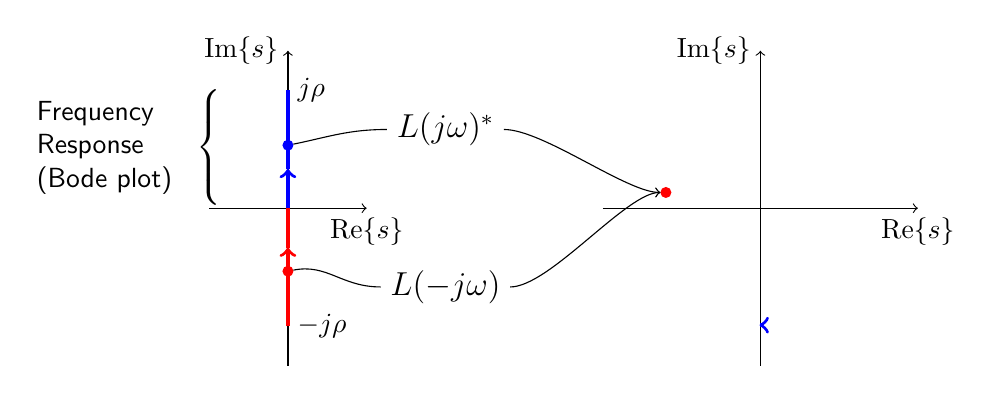
\begin{tikzpicture}[
sysblock/.style={draw,rectangle,inner sep=6pt,minimum width=1.25cm,minimum height=1.0cm,very thick},
summer/.style={circle,draw,very thick}]

\draw[->] (-4,-2) -- ++(0,4) node[left] {Im$\{s\}$};
\draw[->] (-5,0) -- ++(2,0) node[below] {Re$\{s\}$};
\draw[->,very thick,color=blue] (-4,0) -- (-4,.5); 
\draw[very thick,color=blue] (-4,.5) -- (-4,1.5);
\draw[->,very thick,color=red] (-4,-1.5) -- (-4,-.5); 
\draw[very thick,color=red] (-4,-.5) -- (-4,0); 

\draw (-4,1.5) node {\rule{4pt}{0pt}} node[right] {$j\rho$};
\draw (-4,-1.5) node {\rule{4pt}{0pt}} node[right] {$-j\rho$};
%\draw (-4,0) node[circle,fill,inner sep=0pt,outer sep=0pt,color=green] {\rule{4pt}{0pt}};
\draw (-4,.8) node[circle,fill,inner sep=0pt,outer sep=0pt,color=blue] (p1) {\rule{4pt}{0pt}};
\draw (-4,-.8) node[circle,fill,inner sep=0pt,outer sep=0pt,color=red] (p3) {\rule{4pt}{0pt}};
\draw (0.8,0.2) node[circle,fill,inner sep=0pt,outer sep=0pt,color=red] (p2) {\rule{4pt}{0pt}};
\draw (-2,1) node (L) {\large $L(j\omega)^{*}$};
\draw (-2,-1) node (L2) {\large $L(-j\omega)$};
\draw (p1) .. controls ++(.5,.1) and ++(-.5,0) .. (L.180);
\draw[->] (L.0) .. controls ++(.5,0) and ++(-.5,0) .. (p2);

\draw (p3) .. controls ++(.5,.1) and ++(-.5,0) .. (L2.180);
\draw[->] (L2.0) .. controls ++(.5,0) and ++(-.5,0) .. (p2);

\draw (-6,.8) node {\begin{minipage}{.75in}\textsf{Frequency Response (Bode plot)}\end{minipage} $\left\{\rule{0in}{.35in}\right.$};

\draw[->] (0,0) -- ++(4,0) node[below] {Re$\{s\}$};
\draw[->] (2,-2) -- ++(0,4) node[left] {Im$\{s\}$};

\draw[color=blue,very thick] plot[smooth] file {figures/nyquistmapping1.table};
\draw[color=red,very thick] plot[smooth] file {figures/nyquistmapping2.table};
\draw[->,very thick,color=blue] (2,-1.485) -- ++(-.01,0);

%\draw (2,.026) node[circle,fill,inner sep=0pt,outer sep=0pt,color=yellow] {\rule{4pt}{0pt}} ;
%\draw (3.4,0) node[circle,fill,inner sep=0pt,outer sep=0pt,color=green] {\rule{4pt}{0pt}};




\end{tikzpicture}
\end{center}
\end{frame}

\section{Example}

Let's use the Nyquist stability criterion to determine if the following feedback system is stable:

\begin{frame}{Example feedback system}
\begin{center}
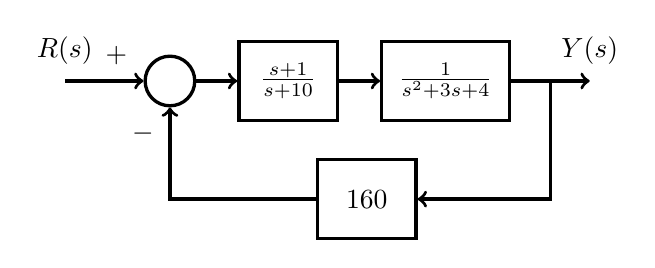
\begin{tikzpicture}[very thick,
sysblock/.style={draw,rectangle,inner sep=6pt,minimum width=1.25cm,minimum height=1.0cm,very thick},
summer/.style={circle,draw,very thick}]

\draw (0,0) node[summer] (sum) {\rule{10pt}{0pt}};
\draw (1.5,0) node[sysblock] (C) {$\frac{s+1}{s+10}$};


\draw (3.5,0) node[sysblock] (G) {$\frac{1}{s^2+3s+4}$};

\draw (2.5,-1.5) node[sysblock] (H) {$160$};

\draw[<-] (sum.180) node[above left=2pt] {$+$} -- ++(-1,0) node[above=2pt] {$R(s)$};
\draw[->] (sum.0) -- (C.180);
\draw[->] (C.0) -- (G.180);
\draw[->] (G.0) -- ++(0.5,0) |- (H.0);
\draw[->] (H.180)  -| (sum.-90) node[below left=2pt] {$-$};
\draw[->] (G.0) ++(0.5,0) -- ++(0.5,0) node[above=2pt] {$Y(s)$};

\end{tikzpicture}
\end{center}
In this case, the loop gain is
\[
L(s) = 160\frac{1}{s^{2}+3s+4}\frac{s+1}{s+10}
\]

\end{frame}
\begin{itemize}
\item Step 1: Determine P, the number of unstable poles of $L(s)$. In this case, all of our open loop transfer functions ($C(s)$, $G(s)$, and $H(s)$) are stable, so $P=0$.
\item Step 2: Draw Nyquist plot. In order to draw the Nyquist plot, we need to know $L(j\omega)$. If $L(s)$ is given to us as a function, this can be done either by hand or using \textsc{Matlab}. Alternatively, we may get this data from an experiment. Let's draw the Bode plot by hand first, and then compare it to a plot from \textsc{Matlab}
\begin{itemize}
\item Bode plot by hand. First, factor out the constant terms in $L(s)$:
\[
L(s) = 4\frac{s+1}{\left(\frac{s^{2}}{4}+\frac{3}{4}s+1\right)\left(\frac{s}{10}+1\right)}
\]
List the break frequencies
\begin{center}
\begin{tabular}{llll}
\toprule
Break Frequency & Item (P/Z? L/RHP? \#?) & Magnitude Slope & Phase Slope\\\midrule
1 rad/s & 1 LHP zero & 20 dB/dec & 45$^{\circ}$/dec \\
2 rad/s & 2 LHP poles & -40 dB/dec &  -90$^{\circ}$/dec \\
10 rad/s & 1 LHP pole & -20 dB/dec & -45$^{\circ}$/dec \\\bottomrule
\end{tabular}
\end{center}
The low frequency term is $4$, so we start the magnitude plot with a zero slope at $20\log(4)=12$ dB, then follow the instructions in the table above at each break frequency
\begin{frame}{Magnitude Plot}
\begin{center}
\begin{tikzpicture}
\draw (0,0) node {\includegraphics[width=3in]{figures/examplemagplot}};
\end{tikzpicture}
\end{center}
\end{frame}

Similarly, a low frequency term without integrators means that the low frequency phase starts at $0^{\circ}$. We add lines for the regions where each term has a non-zero phase slope, and then follow those directions.
\begin{frame}{Phase Plot}
\begin{center}
\begin{tikzpicture}
\draw (0,0) node {\includegraphics[width=3in]{figures/examplephaseplot}};
\draw[thick,*-*] (-2.15,2.1) -- node[pos=.1,above left] {45$^{\circ}$/dec} ++(3.75,0);
\draw[thick,*-*] (-1.63,2.3) -- node[pos=.1,above] {-90$^{\circ}$/dec} ++(3.75,0);
\draw[thick,*-*] (-0.37,2.5) -- node[pos=.2,above] {-45$^{\circ}$/dec} ++(3.75,0);
\end{tikzpicture}
\end{center}
\end{frame}
\item Bode plot from MATLAB
\begin{frame}{Bode Plot}
\begin{center}
\includegraphics[width=2.5in]{figures/examplebodeplot_1}\\
\includegraphics[width=2.5in]{figures/examplebodeplot_2}
\end{center}
\end{frame}
\end{itemize}
Regardless of which method we use, we start by picking points off of the Bode plot, starting with low frequencies. From the Bode plot, we can read off magnitude in decibels, and phase in degrees. 

\begin{frame}{Determine Magnitude and Phase at convenient set of frequencies}
\begin{center}
\begin{minipage}{2in}
\hspace{-.45in}
\begin{tikzpicture}
\draw (0,0) node {\includegraphics[width=2in]{figures/examplebodeplot_1}};
\draw (-1.37,.65) node[circle,fill,inner sep=0pt,outer sep=0pt,color=green] {\rule{4pt}{0pt}};
\draw (-0.2,.7) node[circle,fill,inner sep=0pt,outer sep=0pt,color=cyan] {\rule{4pt}{0pt}};
\draw (.155,.73) node[circle,fill,inner sep=0pt,outer sep=0pt,color=red] {\rule{4pt}{0pt}};
\draw (.63,.61) node[circle,fill,inner sep=0pt,outer sep=0pt,color=yellow] {\rule{4pt}{0pt}};
\draw (1,.48) node[circle,fill,inner sep=0pt,outer sep=0pt,color=orange] {\rule{4pt}{0pt}};
\draw (1.72,.1) node[circle,fill,inner sep=0pt,outer sep=0pt,color=purple] {\rule{4pt}{0pt}};
\draw (2.2,-.15) node[circle,fill,inner sep=0pt,outer sep=0pt,color=black] {\rule{4pt}{0pt}};
\draw (0,-3) node {\includegraphics[width=2in]{figures/examplebodeplot_2}};
\draw (-1.37,-2.4) node[circle,fill,inner sep=0pt,outer sep=0pt,color=green] {\rule{4pt}{0pt}};
\draw (-0.2,-2.45) node[circle,fill,inner sep=0pt,outer sep=0pt,color=cyan] {\rule{4pt}{0pt}};
\draw (.155,-2.7) node[circle,fill,inner sep=0pt,outer sep=0pt,color=red] {\rule{4pt}{0pt}};
\draw (.63,-3.08) node[circle,fill,inner sep=0pt,outer sep=0pt,color=yellow] {\rule{4pt}{0pt}};
\draw (1,-3.35) node[circle,fill,inner sep=0pt,outer sep=0pt,color=orange] {\rule{4pt}{0pt}};
\draw (1.72,-3.62) node[circle,fill,inner sep=0pt,outer sep=0pt,color=purple] {\rule{4pt}{0pt}};
\draw (2.2,-3.7) node[circle,fill,inner sep=0pt,outer sep=0pt,color=black] {\rule{4pt}{0pt}};
\end{tikzpicture}
\end{minipage}
\hspace{-.35in}
\begin{minipage}{2.3in}
\begin{tabular}{cccc}
\small Freq (rad/s) & Mag (dB) & Mag & Phase \\\hline
{\color{green} .1} & 12 & 4.0 & -0.8$^{\circ}$ \\
{\color{cyan} 1 } & 14 & 5.0 & -6$^{\circ}$ \\
{\color{red} 2} & 15 & 5.6 & -38$^{\circ}$ \\
{\color{yellow} 5} & 9 & 2.8 & -92$^{\circ}$ \\
{\color{orange} 10} & 1 & 1.1 & -123$^{\circ}$ \\
{\color{purple} 40} & -20 & 0.10 & -163$^{\circ}$ \\
100 & -36 &  0.015 & -173$^{\circ}$
\end{tabular}
\end{minipage}
\end{center}
\end{frame}

To plot the Nyquist plot, we will need to convert magnitude in decibels back to ``regular'' magnitude. Since the conversion from magnitude M to decibels D is
\[
D = 20\log_{10}M
\]
the inverse mapping will be
\[
M = 10^{D/20}.
\]
For example, looking at the first row of the table above, at 0.1 rad/s the magnitude from the Bode plot is 12 dB. This corresponds to a linear magnitude of  $10^{12/20} = 4$, which is written in the 3rd column.

\begin{frame}{Transfer that information to the complex plane}
\begin{center}
\begin{minipage}{1.5in}
\begin{tabular}{cc}
Mag & Phase \\\hline
{\color{green}  4.0} & {\color{green} -0.8$^{\circ}$ }\\
{\color{cyan} 5.0 }& {\color{cyan}-6$^{\circ}$} \\
{\color{red}  5.6} & {\color{red}   -38$^{\circ}$} \\
{\color{yellow}  2.8} & {\color{yellow} -92$^{\circ}$} \\
{\color{orange} 1.1 }& {\color{orange}-123$^{\circ}$} \\
{\color{purple} 0.10} & {\color{purple}-163$^{\circ}$} \\
  0.015 & -173$^{\circ}$
\end{tabular}
\end{minipage}
\begin{minipage}{2.6in}
\begin{tikzpicture}[scale=.5]
\draw[->] (-2,0) -- (8,0) node[below] {Re$\{s\}$};
\draw[->] (0,-6) -- (0,6) node[left] {Im$\{s\}$};
\draw (-1,-.1) node[below=-3pt] {\tiny $-1$} -- ++(0,.2);
\draw (1,-.1) node[below=-3pt] {\tiny $1$} -- ++(0,.2);
\draw (.1,1) node[right=-3pt] {\tiny $j$} -- ++(-.2,0);
\draw (.1,-1) node[right=-3pt] {\tiny -$j$} -- ++(-.2,0);
\draw (0:4) node[circle,fill,inner sep=0pt,outer sep=0pt,color=green] {\rule{4pt}{0pt}};
\draw (-5:6.3) node[circle,fill,inner sep=0pt,outer sep=0pt,color=cyan] {\rule{4pt}{0pt}};
\draw (-40:8) node[circle,fill,inner sep=0pt,outer sep=0pt,color=red] {\rule{4pt}{0pt}};
\draw (-90:3) node[circle,fill,inner sep=0pt,outer sep=0pt,color=yellow] {\rule{4pt}{0pt}};
\draw (-130:1) node[circle,fill,inner sep=0pt,outer sep=0pt,color=orange] {\rule{4pt}{0pt}};
\draw (-160:0.1) node[circle,fill,inner sep=0pt,outer sep=0pt,color=purple] {\rule{4pt}{0pt}};
\draw (-175:0.018) node[circle,fill,inner sep=0pt,outer sep=0pt,color=black] {\rule{4pt}{0pt}};
\end{tikzpicture}
\end{minipage}
\end{center}
\end{frame}



\begin{frame}{Draw connecting lines, going from low frequency to high frequency}
\begin{center}
\begin{minipage}{1.5in}
\begin{tabular}{cc}
Mag & Phase \\\hline
{\color{green}  4.0} & {\color{green} -0.8$^{\circ}$ }\\
{\color{cyan} 5.0 }& {\color{cyan}-6$^{\circ}$} \\
{\color{red}  5.6} & {\color{red}   -38$^{\circ}$} \\
{\color{yellow}  2.8} & {\color{yellow} -92$^{\circ}$} \\
{\color{orange} 1.1 }& {\color{orange}-123$^{\circ}$} \\
{\color{purple} 0.10} & {\color{purple}-163$^{\circ}$} \\
  0.015 & -173$^{\circ}$
\end{tabular}
\end{minipage}
\begin{minipage}{2.6in}
\begin{tikzpicture}[scale=.5,decoration={markings,mark=at position .6 with {\arrow[blue,very thick]{>}}}]
\draw[->] (-2,0) -- (8,0) node[below] {Re$\{s\}$};
\draw[->] (0,-6) -- (0,6) node[left] {Im$\{s\}$};
\draw (-1,-.1) node[below=-3pt] {\tiny $-1$} -- ++(0,.2);
\draw (1,-.1) node[below=-3pt] {\tiny $1$} -- ++(0,.2);
\draw (.1,1) node[right=-3pt] {\tiny $j$} -- ++(-.2,0);
\draw (.1,-1) node[right=-3pt] {\tiny -$j$} -- ++(-.2,0);
\draw (0:4) node[circle,fill,inner sep=0pt,outer sep=0pt,color=green] (a) {\rule{4pt}{0pt}};
\draw (-5:6.3) node[circle,fill,inner sep=0pt,outer sep=0pt,color=cyan] (b) {\rule{4pt}{0pt}};
\draw (-40:8) node[circle,fill,inner sep=0pt,outer sep=0pt,color=red] (c) {\rule{4pt}{0pt}};
\draw (-90:3) node[circle,fill,inner sep=0pt,outer sep=0pt,color=yellow] (d) {\rule{4pt}{0pt}};
\draw (-130:1) node[circle,fill,inner sep=0pt,outer sep=0pt,color=orange] (e) {\rule{4pt}{0pt}};
\draw (-160:0.1) node[circle,fill,inner sep=0pt,outer sep=0pt,color=purple] (f) {\rule{4pt}{0pt}};
\draw (-175:0.018) node[circle,fill,inner sep=0pt,outer sep=0pt,color=black] (g) {\rule{4pt}{0pt}};
\draw[very thick,color=blue,postaction={decorate}] (a)  .. controls ++(0:.5) and ++(120:.5) .. (b) .. controls ++(-60:.5) and ++(45:.5) .. (c) .. controls ++(180:1) and ++(-45:1) .. (d)  .. controls ++(135:.5) and ++(-90:.5) .. (e) .. controls ++(90:.3) and ++(-180:.3) .. (f);
\end{tikzpicture}
\end{minipage}
\end{center}
\end{frame}

\begin{frame}{Draw Mirror Image to Complete Nyquist Plot}
\begin{center}
\begin{tikzpicture}[scale=.5]
\draw[->] (-2,0) -- (8,0) node[below] {Re$\{s\}$};
\draw[->] (0,-6) -- (0,6) node[left] {Im$\{s\}$};
\draw (-1,-.1) node[below=-3pt] {\tiny $-1$} -- ++(0,.2);
\draw (1,-.1) node[below=-3pt] {\tiny $1$} -- ++(0,.2);
\draw (.1,1) node[right=-3pt] {\tiny $j$} -- ++(-.2,0);
\draw (.1,-1) node[right=-3pt] {\tiny -$j$} -- ++(-.2,0);
\draw (0:4) node[circle,fill,inner sep=0pt,outer sep=0pt,color=green] (a) {\rule{4pt}{0pt}};
\draw (-5:6.3) node[circle,fill,inner sep=0pt,outer sep=0pt,color=cyan] (b) {\rule{4pt}{0pt}};
\draw (-40:8) node[circle,fill,inner sep=0pt,outer sep=0pt,color=red] (c) {\rule{4pt}{0pt}};
\draw (-90:3) node[circle,fill,inner sep=0pt,outer sep=0pt,color=yellow] (d) {\rule{4pt}{0pt}};
\draw (-130:1) node[circle,fill,inner sep=0pt,outer sep=0pt,color=orange] (e) {\rule{4pt}{0pt}};
\draw (-160:0.1) node[circle,fill,inner sep=0pt,outer sep=0pt,color=purple] (f) {\rule{4pt}{0pt}};
\draw (-175:0.018) node[circle,fill,inner sep=0pt,outer sep=0pt,color=black] (g) {\rule{4pt}{0pt}};
\draw[very thick,color=blue,postaction={decorate,decoration={markings,mark=at position .6 with {\arrow[blue,very thick]{>}}}}] (a)  .. controls ++(0:.5) and ++(120:.5) .. (b) .. controls ++(-60:.5) and ++(45:.5) .. (c) .. controls ++(180:1) and ++(-45:1) .. (d) .. controls ++(135:.5) and ++(-90:.5) .. (e) .. controls ++(90:.3) and ++(-180:.3) .. (f);
\draw (0:4) node[color=blue,inner sep=0pt,outer sep=0pt] (aa) {\rule{0pt}{0pt}};
\draw (5:6.3) node[circle,fill,color=blue,inner sep=0pt,outer sep=0pt] (bb) {\rule{0pt}{0pt}};
\draw (40:8) node[circle,fill,color=blue,inner sep=0pt,outer sep=0pt] (cc) {\rule{0pt}{0pt}};
\draw (90:3) node[circle,fill,color=blue,inner sep=0pt,outer sep=0pt] (dd) {\rule{0pt}{0pt}};
\draw (130:1) node[circle,fill,color=blue,inner sep=0pt,outer sep=0pt] (ee) {\rule{0pt}{0pt}};
\draw (160:0.1) node[circle,fill,color=blue,inner sep=0pt,outer sep=0pt] (ff) {\rule{0pt}{0pt}};
\draw (175:0.018) node[circle,fill,color=blue,inner sep=0pt,outer sep=0pt] (gg) {\rule{4pt}{0pt}};
\draw[very thick,color=blue,postaction={decorate,decoration={markings,mark=at position .6 with {\arrowreversed[blue,very thick]{>}}}}] (aa)  .. controls ++(0:.5) and ++(-120:.5) .. (bb) .. controls ++(60:.5) and ++(-45:.5) .. (cc) .. controls ++(-180:1) and ++(45:1) .. (dd) .. controls ++(-135:.5) and ++(90:.5) .. (ee) .. controls ++(-90:.3) and ++(180:.3) .. (ff);
\end{tikzpicture}
\end{center}
\end{frame}

\item Note that the Nyquist plot does not go through $-1+j0$, thus the closed loop system has no poles on the $j\omega$ axis. Count number of encirclements of $-1+j0$ by Nyquist plot. 
\begin{frame}{Determine Number of Clockwise Encirclements}
\begin{center}
\begin{tikzpicture}[scale=.5]
\draw[->] (-2,0) -- (8,0) node[below] {Re$\{s\}$};
\draw[->] (0,-6) -- (0,6) node[left] {Im$\{s\}$};
\draw (-1,-.1) node[below=-3pt] {\tiny $-1$} -- ++(0,.2);
\draw (1,-.1) node[below=-3pt] {\tiny $1$} -- ++(0,.2);
\draw (.1,1) node[right=-3pt] {\tiny $j$} -- ++(-.2,0);
\draw (.1,-1) node[right=-3pt] {\tiny -$j$} -- ++(-.2,0);
\draw (0:4) node[circle,fill,inner sep=0pt,outer sep=0pt,color=green] (a) {\rule{4pt}{0pt}};
\draw (-5:6.3) node[circle,fill,inner sep=0pt,outer sep=0pt,color=cyan] (b) {\rule{4pt}{0pt}};
\draw (-40:8) node[circle,fill,inner sep=0pt,outer sep=0pt,color=red] (c) {\rule{4pt}{0pt}};
\draw (-90:3) node[circle,fill,inner sep=0pt,outer sep=0pt,color=yellow] (d) {\rule{4pt}{0pt}};
\draw (-130:1) node[circle,fill,inner sep=0pt,outer sep=0pt,color=orange] (e) {\rule{4pt}{0pt}};
\draw (-160:0.1) node[circle,fill,inner sep=0pt,outer sep=0pt,color=purple] (f) {\rule{4pt}{0pt}};
\draw (-175:0.018) node[circle,fill,inner sep=0pt,outer sep=0pt,color=black] (g) {\rule{4pt}{0pt}};
\draw[very thick,color=blue,postaction={decorate,decoration={markings,mark=at position .6 with {\arrow[blue,very thick]{>}}}}] (a)  .. controls ++(0:.5) and ++(120:.5) .. (b) .. controls ++(-60:.5) and ++(45:.5) .. (c) .. controls ++(180:1) and ++(-45:1) .. (d) .. controls ++(135:.5) and ++(-90:.5) .. (e) .. controls ++(90:.3) and ++(-180:.3) .. (f);
\draw (0:4) node[color=blue,inner sep=0pt,outer sep=0pt] (aa) {\rule{0pt}{0pt}};
\draw (5:6.3) node[circle,fill,color=blue,inner sep=0pt,outer sep=0pt] (bb) {\rule{0pt}{0pt}};
\draw (40:8) node[circle,fill,color=blue,inner sep=0pt,outer sep=0pt] (cc) {\rule{0pt}{0pt}};
\draw (90:3) node[circle,fill,color=blue,inner sep=0pt,outer sep=0pt] (dd) {\rule{0pt}{0pt}};
\draw (130:1) node[circle,fill,color=blue,inner sep=0pt,outer sep=0pt] (ee) {\rule{0pt}{0pt}};
\draw (160:0.1) node[circle,fill,color=blue,inner sep=0pt,outer sep=0pt] (ff) {\rule{0pt}{0pt}};
\draw (175:0.018) node[circle,fill,color=blue,inner sep=0pt,outer sep=0pt] (gg) {\rule{4pt}{0pt}};
\draw[very thick,color=blue,postaction={decorate,decoration={markings,mark=at position .6 with {\arrowreversed[blue,very thick]{>}}}}] (aa)  .. controls ++(0:.5) and ++(-120:.5) .. (bb) .. controls ++(60:.5) and ++(-45:.5) .. (cc) .. controls ++(-180:1) and ++(45:1) .. (dd) .. controls ++(-135:.5) and ++(90:.5) .. (ee) .. controls ++(-90:.3) and ++(180:.3) .. (ff);
\draw (12,0) node {$N=0$};
\end{tikzpicture}
\end{center}
\end{frame}
\item Number of {\em closed loop} poles with positive real part is $Z=P+N$. Thus
\[
Z= 0 + 0 =0
\]
This tells us that there are {\em no} unstable closed loop poles, and the closed loop system is {\em stable}.
\end{itemize}

\section{Nyquist Plots using \textsc{Matlab}}

In \textsc{Matlab} if the open loop system $G(s)$ is defined to be the variable \texttt{sys}, then the Nyquist plot can be found using the command \texttt{nyquist(sys)}. As an example, the Nyquist plot for the example in the previous section can be created using the commands:

\begin{frame}{Nyquist Plot using \textsc{Matlab}}
\noindent\texttt{>> C = tf([1 1],[1 10]);\\<all>
>> G = tf(1,[1 3 4]);\\<all>
>> H = 160;\\<all>
>> nyquist(H*G*C)}
\begin{center}
\includegraphics[width=3in]{figures/matlabnyquist}
\end{center}
\end{frame}

Note that the point $-1+j0$ is marked with a red square.

\section{Lecture Highlights}
The primary takeaways from this article include
\begin{enumerate}
\setlength{\itemsep}{5pt}
\setlength{\parskip}{0pt}
\setlength{\parsep}{0pt}
\item The Nyquist stability test is another test to check for stability. 
\item The Nyquist test uses information derived from the \textit{open loop} frequency response (Bode plot) to determine if the \textit{closed loop} transfer function is stable.
\item The Nyquist test can tell you how many unstable closed loop poles a system has.
\item When creating a Nyquist plot from a Bode plot, a common mistake is forgetting to convert from the magnitude in dB (which is found in the Bode plot) to the magnitude gain.
\end{enumerate}


\section{Quiz Yourself}

\subsection{Questions}

For these problems, we will be using the unity gain feedback configuration
\begin{center}
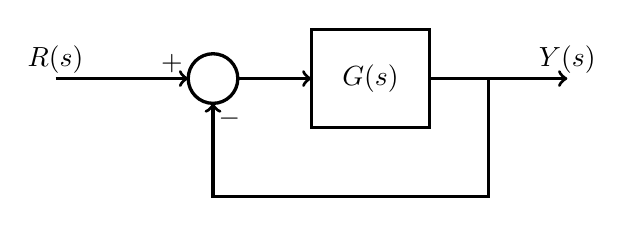
\begin{tikzpicture}[scale=1,inner sep=0pt,outer sep=0pt,very thick,
sysblock/.style={draw,rectangle,inner sep=2pt,minimum width=1.5cm,minimum height=1.25cm,very thick}]
\draw (2,0) node[draw,circle] (sum1) {$\rule{0pt}{18pt}$};
\draw (4,0) node[sysblock] (Kp) {$G(s)$};
\draw[->] (0,0) node[above=2pt] {$R(s)$} -- (sum1.180) node[above left=2pt] {$+$};
\draw[->] (sum1.0) --  (Kp);
\draw[->] (Kp) -- ++(2.5,0) node[above=2pt] {$Y(s)$};
\draw[->] (Kp) ++(1.5,0) -- ++(0,-1.5) -| (sum1.-90) node[below right=2pt] {$-$};
\end{tikzpicture}
\end{center}

\begin{enumerate}
\setlength{\itemsep}{5pt}
\setlength{\parskip}{0pt}
\setlength{\parsep}{0pt}
\item Find the Nyquist plot if $G(s)$ has the following Bode plot
\begin{center}
\includegraphics[width=5in]{quizfigures/prob1}
\end{center}
This system is open loop stable. Will it be closed loop stable?
\item Find the Nyquist plot for the system
\[
G(s) = \frac{(s-100)}{(s+1)(s+10)}
\]
Compare your results to \textsc{Matlab}. How many unstable poles does the closed loop system have? 
\end{enumerate}



\subsection{Solutions}
\begin{enumerate}
\setlength{\itemsep}{5pt}
\setlength{\parskip}{0pt}
\setlength{\parsep}{0pt}
\item \rule{12pt}{0pt}
\begin{center}
\includegraphics[width=6in]{quizfigures/1asoln}\\
\end{center}
\item \rule{12pt}{0pt}
\begin{center}
\includegraphics[width=5in]{quizfigures/2asoln}\\
\includegraphics[width=6in]{quizfigures/2bsoln}\\
\end{center}
\texttt{>> s=tf([1 0],1)\\
>> nyquist((s-100)/((s+1)*(s+10)))}\\
\begin{center}
\includegraphics[width=5in]{quizfigures/2csoln}
\end{center}
\end{enumerate}


\end{document}


